\documentclass[ENG]{TFUOC}%IB: CASTELLÀ, CAT: CATALÀ, ENG: ANGLISH

%Other packages
\usepackage{hyperref}

%Introduce Work Data
\title{Functional Characterization of lncRNA Biomarkers in Colorectal Cancer Using RiNALMo}
\titcrt{Very short title} %Short title to appear in header
\author{Salomon Elieser Marquez Villalobos}
\date{\today}

\nomPDC{Fernando Pastor and Igor Ruiz}
\nomPRA{Diego Garrido Martin}
\titulac{Master in Bioinformatics and Bioestadistics}
\area{M0.207 Omics Data Analysis}
\idioma{English}
\credits{15}
\parcla{CRC, biomarkers, AI}

\licenc{ccBy}
%Possible licenses
%ccByNcNd
%ccByNcSa
%ccByNc
%ccByNd
%ccBySa
%ccBy
%GNU
%copyright


%%%%%%%%%%
% Summary in language

%\abstractidioma{
%Maximum 250 words, for the purpose, context of application, methodology, results and conclusions of the work.
%}

% Summary in English.
%\abstractenglish{
%A maximum of 250 words, detailing the purpose, context of application, methodology, results and conclusions of the work.
%}

\begin{document}

\estructura

%\tableofcontents

%\listoffigures

%\listoftables

\chapter{Introduction}

\section{Context and justification of the project}

\textit{Colorectal cancer (CRC) is caused by a sequence of somatic genomic alterations affecting driver genes in core cancer pathways} \cite{vogelsteinCancerGenomeLandscapes2013}. CRC is the third most common malignancy and a leading cause of cancer-related death globally, with a rising incidence in younger individuals, early-onset colorectal cancer (EOCRC \textless 50 years old) patients versus later-onset colorectal cancer (LOCRC \textgreater 50 years old) patients \cite{marxIdentificationDifferentiallyExpressed2024}. 
The development of CRC is driven by the accumulation of genomic alterations in key oncogenic and tumor-suppressive pathways, including WNT, RAS-MAPK, PI3K, and $TGF-\beta$ \cite{nunesPrognosticGenomeTranscriptome2024}. While large-scale sequencing efforts have successfully identified numerous protein-coding driver genes, the functional role of the non-coding genome remains a critical and largely unexplored frontier in CRC biology.

Long non-coding RNAs (lncRNAs) are regulatory RNA molecules longer than 200 nucleotides that are not translated into proteins but exert their function as RNA. They are key regulators of gene expression, participating in chromatin architecture, transcription, and splicing. Their highly cell- and tissue-specific expression patterns make them excellent candidates for cancer biomarkers and therapeutic targets. However, some traditional bioinformatics pipelines for biomarker discovery have biased against lncRNAs. For instance, methods that rely on protein-protein interaction (PPI) networks, such as the one used by \cite{vaziri-moghadamIntegratingMachineLearning2024}, exclude non-coding genes from their analysis.

This limitation is being overcome by comprehensive whole-genome sequencing (WGS) studies, which analyze the entire genome without a bias toward coding regions. Recent landmark studies by \cite{cornishGenomicLandscape20232024a} and \cite{nunesPrognosticGenomeTranscriptome2024} have cataloged thousands of genomic alterations in CRC to identify novel drivers. These efforts have successfully identified non-coding candidates with high-confidence, \textit{involving the lincRNA LINC00673 (also known as LINC00511), a transcript that interacts with the CRC driver genes EZH2 and PTPN11} \cite{cornishGenomicLandscape20232024a}, highlighting them as promising but functionally uncharacterized players in CRC.

The critical gap in the field is no longer just the discovery of these lncRNAs, but the understanding of their molecular function. This project is justified by the opportunity to address this gap directly by applying a state-of-the-art computational tool. We will leverage RiNALMo (RiboNucleic Acid Language Model), a new 650M-parameter language model pre-trained on 36 million non-coding RNA sequences \cite{penicRiNALMoGeneralpurposeRNA2025}. RiNALMo has achieved state-of-the-art results on downstream tasks like secondary structure prediction, non-coding RNA (ncRNA) family classification, splice-site prediction, mean ribosome loading (MRL), translation efficiency (TE), and expression level (EL) prediction.


\section{Work objectives}

\subsection{General objective}
The primary objective of this thesis is to characterize the structure and function of lncRNA candidates previously identified in colorectal cancer, using the state-of-the-art RiNALMo language model.

\subsection{Specific objectives}

\begin{enumerate}
    \item To perform a literature review to select and curate a list of lncRNA candidates with strong evidence of association with CRC (e.g., LINC00673, PWRN1 from \cite{cornishGenomicLandscape20232024a}).
    \item To establish a robust computational environment on a high-performance computing (HPC) cluster or a cloud-based platform for application of the RiNALMo model. 
    \item To apply RiNALMo model to the prioritized CRC-associated lncRNA candidates to generate predictions about their secondary structure, ncRNA family, and splice-site.
    \item To analyze and interpret the predicted structures to formulate functional hypotheses regarding their molecular mechanisms in CRC.
\end{enumerate}

\section{Focus and method followed}

Given the reduced 3-month timeframe, this project will focus on the functional characterization of known candidates using RiNALMo.  	

\begin{itemize}
    \item \textbf{Phase 1: Candidate Selection and Pipeline Preparation (October)}. This phase will focus on rapidly establishing the project's foundation.
    \begin{enumerate}
        \item Candidate Selection: High-confidence lncRNA candidates (LINC00673, PWRN1) will be selected based on their identification as putative non-coding drivers in the \cite{cornishGenomicLandscape20232024a} study. Their sequences will be retrieved from genomic databases (e.g., Ensembl).
        \item Computational Environment Setup: Access to a suitable HPC cluster (e.g., at University of Navarra) or a cloud platform (e.g., Modal) will be secured. A reproducible software environment will be built using Conda or Singularity containers, including Python, PyTorch, and specialized libraries like FlashAttention-2. The lightweight version of RiNALMo (35M params) codebase and pre-trained weights will be downloaded from \href{https://github.com/lbcb-sci/RiNALMo}{RiNALMo GitHub Repository} and installed, as specified by the authors.
        \item Pipeline Validation: The quickstart guide of the lightweighted version of RiNALMo will be run for inference of a few RNA sequences to validate the entire computational pipeline.
    \end{enumerate}
    \item \textbf{Phase 2: Downstream tasks and Functional Prediction (November)} This phase will execute the core computational work of the thesis.
    \begin{enumerate}
        \item Secondary Structure Prediction Task: The 35M-parameter RiNALMo model will be executed on the HPC platform to predict the secondary structures of the selected CRC-associated lncRNAs. 
        \item Analysis and Interpretation: The predicted structures will be visualized and analyzed for conserved or notable motifs (e.g., hairpin loops, bulges) that could serve as binding sites for proteins or other RNAs, providing mechanistic hypotheses for their function.
        \item Complete Downstream Tasks: The other downstream tasks will be implemented prioritizing the structure, ncRNA family and splice site prediction ones. 
        \item Increment Model Size: RiNALMo comprises the following sizes: 35M params (micro), 150M params (mega), and 650M params (giga). For the mega and micro sizes, a Tesla P100 node with 12 GB VRAM is required whereas for the giga model, a nice-to-have option would be an L40S node with 48 GB VRAM. Thus, if the UNAV cluster permits, other versions of the model will be explored. 
    \end{enumerate}

\end{itemize}


\section{Working Plan}

\subsection{Tasks}

\begin{enumerate}
    \item Project Setup (Week 1-2: Oct 1-15): Finalize literature review, confirm lncRNA candidates, acquire all necessary data, and apply for HPC access.
    \item Environment and Pipeline Validation (Week 3-4: Oct 16-31): Set up the complete computational environment on the UNAV HPC cluster. Validate that the lightweighted version of RiNALMo is up and running. 
    \item Secondary Structure Prediction (Week 5-6: Nov 1-15): Apply the model to generate secondary structure predictions for the selected CRC lncRNAs. 
    \item Implement Other Downstream Tasks  (Week 7-8: Nov 16-30): Continue the analysis, visualization, and interpretation of results with other downstream tasks and if possible scale up the RiNALMo model size to compare tasks’ performance. 
    \item Thesis Writing and Finalization (Week 9-11: Dec 1-15): Complete the analysis, discuss relevant results and write the full thesis manuscript for submission to the advisors.
    
\end{enumerate}

\subsection{Milestones}
\begin{enumerate}
    \item M1 (by October 31): Computational pipeline fully validated on a small scale on the UNAV HPC cluster.
    \item M2 (by November 30): All primary computational results, including RiNALMo downstream tasks for lncRNA predictions, have been generated and analyzed.
    \item M3 (by December 15): Submission of the final thesis manuscript draft to advisors.
    
\end{enumerate}
\subsection{Risk Analysis}

\begin{table}[htbp]
    \centering
    \caption{Risk Assessment and Mitigation Strategies}
    \label{tab:risk-mitigation}
    \begin{tabular}{p{7cm} p{7cm}}
        \hline
        \textbf{Risk} & \textbf{Mitigation Strategy} \\
        \hline
        1. Time Constraints: The 3-month timeline leaves little room for unexpected delays. &
        The project scope has been narrowed to focus solely on the functional characterization of lncRNAs, eliminating the discovery phase and reusing transcripts already associated with CRC. \\

        2. Delays in HPC Access or Execution: Technical issues on the HPC could delay the execution of the model. &
        Development and pipeline validation will be done on the UNAV HPC cluster. Initially, the secondary structure task will be submitted and monitored closely to resolve any issues promptly. \\

        3. RiNALMo Model/Code Issues: The public release of the model and scripts may have bugs, be delayed, or be difficult to use. &
        Although the \cite{penicRiNALMoGeneralpurposeRNA2025} provides the code and weights of the RiNALMo Model, a backup plan will be prepared to characterize the same lncRNAs using established, less novel tools (e.g., RNAstructure, CONTRAfold) to ensure a completed project. \\

        4. Uninformative Results: The predicted structures may not reveal obvious functional motifs. &
        The primary contribution of this thesis is the novel application of a state-of-the-art methodology to a critical biological problem. The thesis will be framed around the workflow itself, with the interpretation of results forming the discussion, even if they are not immediately conclusive. \\
        \hline
    \end{tabular}
\end{table}


\section{Brief summary of products obtained}

This thesis will deliver a focused, high-impact contribution by being one of the first studies to apply the RiNALMo language model for CRC.

\begin{itemize}
    \item A complete Master's thesis manuscript detailing the workflow, results, and interpretation.
    \item Generation of the first predicted secondary structures for high-confidence CRC-associated lncRNAs like LINC00673 and PWRN1, providing a foundation for future experimental validation.
    \item Documentation of a rapid and powerful workflow for applying large RNA language models to functionally characterize newly discovered non-coding genes from large genomic studies.
    \item A practical demonstration of the feasibility and utility of a foundational RNA model to gain mechanistic insights into cancer biology, moving beyond expression-based biomarker discovery.
    \item All developed scripts and analysis notebooks will be organized and made available in a public repository (e.g., GitHub) to ensure reproducibility.
\end{itemize}
%It is not necessary to enter in detail: the detailed description will be done in the rest of the chapters.

% \section{Brief description of other memory chapters}

% Brief explanation of the contents of each chapter and its relationship with the global project.

%\chapter{State of Art}

%State of the art of the subject in question. It should end up showing why work is important and contributes something, and with the hypotheses of work.

% \chapter{Materials and methods}
% In these sections, it is necessary to describe:
% \begin{itemize}
%     \item The most relevant aspects of the design and development of the work.
%     \item The methodology chosen to carry out this development, describing the possible alternatives, the decisions taken, and the criteria used to make these decisions.
%     \item The products obtained.
% \end{itemize}

 
% \textbf{Chapter structuring may vary depending on the type of work.}  
 
% If applicable, a section on “Economic evaluation of work” will be included. This section will indicate the expenses associated with the development and maintenance of work, as well as the economic benefits obtained and a final analysis on the viability of the product.



% \chapter{Results}

% Detail in this section the results obtained using the methodology described in the previous section.


%Recull of job results. There should be a correspondence with the methodology that the results are what is obtained after applying the methodology.

% The figures must be explained and quoted in the text, such as \ref{fig:my_label}, in which the error is shown depending on the distance, in arbitrary units. All graphs must have the title of the axes.

% \begin{figure}[!htbp]
%     \centering
%     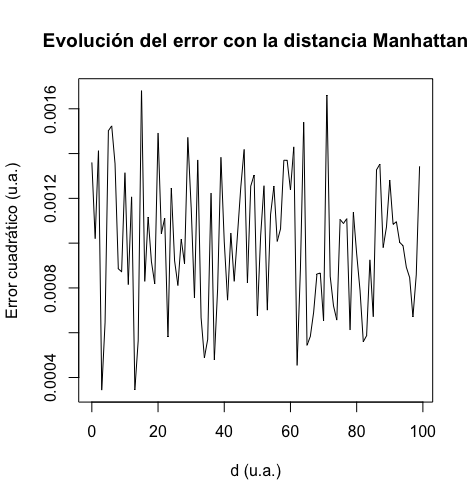
\includegraphics[width=7truecm]{Rplotmanh.png}
%     \caption{Error working distance in arbitrary units.}
%     \label{fig:my_label}
% \end{figure}

%\chapter{Discussion}
%Discussion of results in project context. It is in this section that they make sense and in which the research questions are answered and it is shown how the results respond to the problems raised.

%This part may not apply depending on the type of work.

%\chapter{Economic evaluation}
%If applicable, a section of ``Economic evaluation of work' will be included. This section will indicate the expenses associated with the development and maintenance of work, as well as the economic benefits obtained. A final analysis on the viability of the product must be carried out.

% \chapter{Conclusions and future works}

%\section{Conclusions}
% This chapter must include:
% \begin{itemize}
% \item A description of the conclusions of the work:
% \begin{itemize}
%     \item Once the results have been obtained, what conclusions are drawn?
%     \item Are these results as expected? Or have they been amazing? Why?
% \end{itemize}
% \item A critical reflection on the achievement of the objectives initially set:
% \begin{itemize}
%     \item Have we achieved all the objectives? If the answer is negative, why?
% \end{itemize}
% \item A critical analysis of the monitoring of planning and methodology throughout the product:
% \begin{itemize}
%     \item Has the schedule been followed?
%     \item Has the planned methodology been adequate enough?
%     \item Has it been necessary to introduce changes to ensure the success of the work? Why?
% \end{itemize}
% \item From the impacts foreseen in \ref{s:etic}, ethical-social, sustainability and diversity, evaluate/mention whether they have been mitigated (if they were negative) or whether they have been achieved (if they were positive). 
% \item If unforeseen impacts have appeared in \ref{s:etic}, evaluate/mention how they have mitigated (if they were negative) or what they have contributed (if they were positive).
% \item The future lines of work that have not been explored in this work and have remained pending.


%\item A description of the conclusions of the work: What lessons have been learned from work?
%\item A critical reflection on the achievement of the objectives initially set: Have we achieved all the objectives? If the answer is negative, why?
%\item Of the impacts foreseen in the section \ref{s:etic}, an assessment, or at least mention, of whether they have been mitigated (if they were negative) or whether they have been achieved (if they were positive). 
% \end{itemize}

%\section{Future Lines}
%The future lines of work that could not be explored in this work and have been pending.

%\section{Schedule Tracking}
%A critical analysis of the monitoring of the planning and methodology throughout the work: 
%\begin{itemize}
%    \item  Have the schedule been followed? 
%    \item Has the planned methodology been adequate? 
%    \item Has it been necessary to introduce changes to ensure the success of the work? Why?
%\end{itemize}

% \chapter{Glossary}

% Definition of the most relevant terms and acronyms used in the Report.

%Defining the most relevant terms and acronyms used within the Memory.

\bibliographystyle{unsrt}
\bibliography{references}



% \newpage
% \appendix
% List of sections that are too extensive to include in memory and have a self-contained character (e.g. user manuals, installation manuals, etc.)
 
% Depending on the type of work, there may be no need to add an annex.

\end{document}
